\documentclass[main.tex]{subfiles}
\begin{document}\newpage
\setdoublesep{0.35700 em}  % 'Bond Spacing'
\setatomsep{1.78500 em}    % 'Fixed Length'
\setbondoffset{0.18265 em} % 'Margin Width'
\newcommand{\bondwidth}{0.06642 em} % 'Line Width'
\setbondstyle{line width = \bondwidth}
\newgeometry{left=0.8in,right=0.8in, top=2.5cm,bottom=2cm}
\fancyhfoffset[E,O]{0pt}
\setlength{\columnsep}{30pt}
\begin{conclusion}
\end{conclusion}
\setstretch{0.3}
\begin{multicols*}{2}

{\raggedright\textsc{\textbf{Light }}\par}
\begin{enumerate}

\item Calculate the energy in joules of a radiation with frequency $2.0\times10^{18}$ Hz?
\begin{flushright}\small Ans: $1.32\times10^{-15}$J\end{flushright}

\item Calculate the frequency of a radiation with energy $5.6\times10^{-20}$ J?
\begin{flushright}\small Ans: $8.5\times10^{13}$Hz\end{flushright}

\item Calculate the energy in joules of a radiation with wavelength $653$ nm?
\begin{flushright}\small Ans: $3.03\times10^{-19}$J\end{flushright}

\item Calculate the wavelength of a radiation with  energy $5.34\times10^{-16}$J?
\begin{flushright}\small Ans: $0.37$ nm\end{flushright}

\item Calculate the wavelength of a radiation with  frequency of $3.4\times10^{14}$ Hz?
\begin{flushright}\small Ans: $882$ nm\end{flushright}

\item Indicate the color of a radiation with $\lambda$= 510nm.
\begin{flushright}\small Ans: Green\end{flushright}

\item Indicate the color of a radiation with $\lambda$= 580nm.
\begin{flushright}\small Ans: Yellow\end{flushright}
\item Classify the nature of a radiation with $\gamma$= $3.4\times10^{8}$Hz
\begin{flushright}\small Ans: Microwaves\end{flushright}



\item Sections of two electromagnetic waves A and B  are represented below. Rank them in order of (a) increasing frequency; (b) increasing energy;  (c) If wave B represents visible radiation, is wave A more likely to be IR or UV radiation?  
     \begin{centering}
     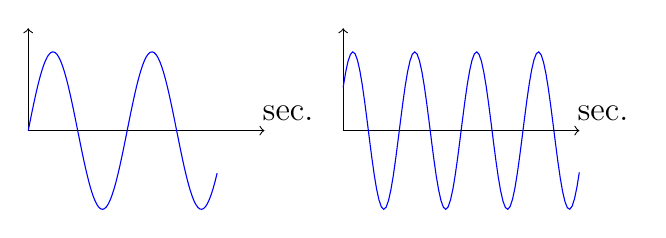
\begin{tikzpicture}[xscale=1,yscale=1]
      \begin{scope}[font=\itshape]
  \draw[->] (0,0) -- (0,1.3);
  \draw[->] (0,0)--(3,0) node[font=\large,black, above, pos = 1.1] {sec.};
  \draw[domain=0:2.4,samples=100,blue] plot(\x,{sin(\x r*5)});
   \draw[->] (4,0) -- (4,1.3);
  \draw[->] (4,0)--(7,0) node[font=\large,black, above , pos = 1.1] {sec.};
  \draw[domain=4:7.0,samples=100,blue] plot(\x,{sin(\x r*8)});
 \end{scope}
\end{tikzpicture}
     \end{centering}
  \begin{flushright}\small Ans: (a) $\gamma_A$<$\gamma_B$; (b) $E_A$<$E_B$; (c) IR \end{flushright}

\item Sections of two electromagnetic waves A and B  are represented below. Rank them in order of (a) increasing wavelength; (b) increasing energy;  (c) If wave B represents visible radiation, is wave A more likely to be IR or UV radiation?  
     \begin{centering}
     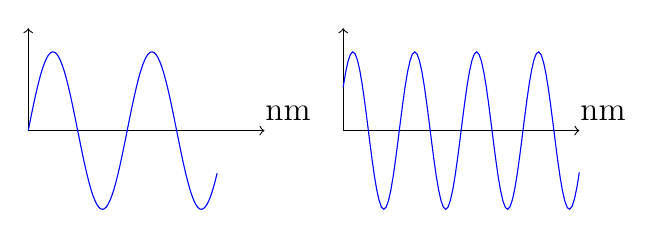
\begin{tikzpicture}[xscale=1,yscale=1]
      \begin{scope}[font=\itshape]
  \draw[->] (0,0) -- (0,1.3);
  \draw[->] (0,0)--(3,0) node[font=\large,black, above, pos = 1.1] {nm};
  \draw[domain=0:2.4,samples=100,blue] plot(\x,{sin(\x r*5)});
   \draw[->] (4,0) -- (4,1.3);
  \draw[->] (4,0)--(7,0) node[font=\large,black, above , pos = 1.1] {nm};
  \draw[domain=4:7.0,samples=100,blue] plot(\x,{sin(\x r*8)});
 \end{scope}
\end{tikzpicture}
     \end{centering}
  \begin{flushright}\small Ans: (a) $\lambda_B$<$\lambda_A$; (b) $E_A$<$E_B$; (c) UV \end{flushright}
    
     
{\raggedright\textsc{\textbf{The atomic spectrum of hydrogen }}\par}

\item Which of these electron transitions correspond to absorption of energy and which to emission?
\begin{enumerate}[label=(\alph*)]\begin{multicols*}{2}
\item $\Delta E_{1\rightarrow 2}$
\item $\Delta E_{2\rightarrow 1}$
\item $\Delta E_{3\rightarrow 1}$
\item  $\Delta E_{3\rightarrow 5}$
\item $\Delta E_{3\rightarrow 5}$
\end{multicols*}\end{enumerate}
  \begin{flushright}\small Ans:  absorption: (a), (d), (e); Emission: (b), (c)  \end{flushright}



\item Use the Bohr equation to  find the energy of the photon emitted when an H atom undergoes a transition from $n=1$ to $n=4$.
  \begin{flushright}\small Ans:  $2.04\times10^{-18}$ J  \end{flushright}

\item Use the Bohr equation to  find the wavelength (in nm) of the photon emitted when an H atom undergoes a transition from $n=2$ to $n=4$.
  \begin{flushright}\small Ans:  $485$ nm \end{flushright}

\item Use the Bohr equation to  find the frequency (in Hz) of the photon emitted when an H atom undergoes a transition from $n=1$ to $n=5$.
  \begin{flushright}\small Ans:  $3.16\times10^{15}$ Hz \end{flushright}


\item An electron in the lowest energy level of H atom absorbs a photon of wavelength 96.97 nm. Indicate the final energy level of the electron moved.
  \begin{flushright}\small Ans:  $n=5$ \end{flushright}

{\raggedright\textsc{\textbf{Quantum mechanics and electronic structure }}\par}


\item Indicate the number of orbitals that can have the following designations: (a) 2s; (b) 3p; (c) 0p; (d) $n=4$?
  \begin{flushright}\small Ans:  (a) two orbitals; (b) 3 orbitals; (c) none; (d) 16 orbitals. \end{flushright}

\item Indicate if the following combination of quantum numbers are allowed:\\
\begin{tabularx}{\columnwidth}{>{}m{.20\linewidth} *{4}{Y} }
  \toprule
\heading{$n$} & \heading{$l$}  &  \heading{$m_1$} & \heading{$m_s$} & \heading{Allowed?}   \\
    \midrule
  4	&	4	&	1	&	$+^1/_2$    \\
   2	&	1&		4	&	$+^1/_2$   \\
4		&2	&	-2	&	$-^1/_2$\\    
    \bottomrule
\end{tabularx}
  \begin{flushright}\small Ans:  no, no, yes. \end{flushright}

\item For each of the following sublevels, give the n and l values and the number of orbitals: (a) 6s; (b) 4d; (c) 2p.
  \begin{flushright}\small Ans: (a) $n=6;l=0$; (b) $n=4;l=2$; (c) $n=2;l=1$. \end{flushright}

\item What is the element with the electron configuration $1s^2 2s^2 2p^6 3s^2 3p^5$?
\begin{enumerate}[label=(\alph*)]\begin{multicols*}{3}
\item Be
\item F
\item Cl
\item  S
\item Ar
\end{multicols*}\flushright  {\small Ans: (c)}
\end{enumerate}

\item What is the element with the electron configuration $1s^2 2s^2 2p^6 3s^2 3p^4$?
\begin{enumerate}[label=(\alph*)]\begin{multicols*}{3}

\item Be
\item F
\item Cl
\item  S
\item Ar
\end{multicols*}\flushright  {\small Ans: (d)}
\end{enumerate}

\item What is the element with the abbreviated electron configuration $[Kr]5s^2 4d^8$?
\begin{enumerate}[label=(\alph*)]\begin{multicols*}{3}

\item Ni
\item Pd
\item Pt
\item  Kr
\item Xe
\end{multicols*}\flushright  {\small Ans: (b)}
\end{enumerate}

{\raggedright\textsc{\textbf{Periodic Properties }}\par}

\item Of the elements:  B, C, F, Li, and Na, the element with the largest atomic radius is
\begin{enumerate}[label=(\alph*)]\begin{multicols*}{3}
\item B
\item C
\item F
\item  Li
\item Na
\flushright  {\small Ans: (e)}
\end{multicols*}\end{enumerate}

\item Of the elements:  B, C, F, Li, and Na, the element with the largest ionization energy is
\begin{enumerate}[label=(\alph*)]\begin{multicols*}{3}
\item B
\item C
\item F
\item  Li
\item Na
\flushright  {\small Ans: (e)}
\end{multicols*}

\end{enumerate}
\item Of the elements:  B, C, F, Li, and Na, the element with the largest electronegativity is
\begin{enumerate}[label=(\alph*)]\begin{multicols*}{3}
\item B
\item C
\item F
\item  Li
\item Na\end{multicols*}\flushright  {\small Ans: (c)}
\end{enumerate}

\item Of the elements:  B, C, F, Li, and Na, the element with the largest metallic character is
\begin{enumerate}[label=(\alph*)]\begin{multicols*}{3}
\item B
\item C
\item F
\item  Li
\item Na
\end{multicols*}\flushright  {\small Ans: (d)}
\end{enumerate}


\restoregeometry
\end{enumerate}
\end{multicols*}
\pagecolor{green!10}\afterpage{\nopagecolor}\newpage
\end{document}

